\documentclass[tikz, border=10pt]{standalone}
\usepackage{pgfplots}
\usepgfplotslibrary{fillbetween}
\pgfplotsset{compat=1.18}

\begin{document}
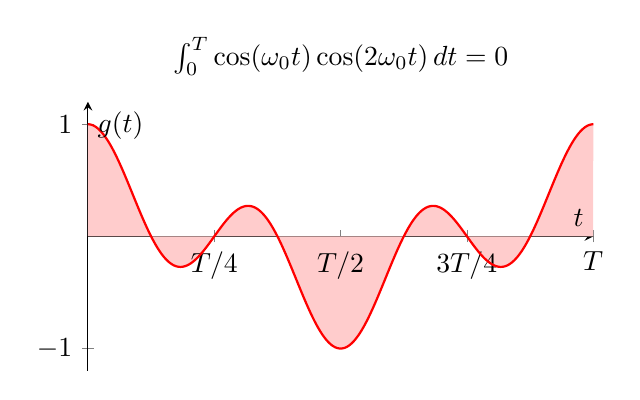
\begin{tikzpicture}
    \begin{axis}[
        width=8cm, height=5cm,
        axis lines=middle,
        xlabel={$t$}, ylabel={$g(t)$},
        xmin=0, xmax=2*pi,
        ymin=-1.2, ymax=1.2,
        xtick={0, 1.57, 3.14, 4.71, 6.28},
        xticklabels={0, $T/4$, $T/2$, $3T/4$, $T$},
        samples=400,
        domain=0:2*pi,
        title={$\int_{0}^{T} \cos(\omega_0 t)\cos(2\omega_0 t) \, dt = 0$}
    ]
        \addplot[name path=f, red, thick] {cos(deg(x))*cos(deg(2*x))};
        \path[name path=axis] (axis cs:0,0) -- (axis cs:6.28,0);
        
        \addplot[red!20] fill between[of=f and axis];
    \end{axis}
\end{tikzpicture}
\end{document}
